%%%%%%%%%%%%%%%%%%%%%%%%%%%%%%%%%%%%%%%%%
% Beamer Presentation
% LaTeX Template
% Version 1.0 (10/11/12)
%
% This template has been downloaded from:
% http://www.LaTeXTemplates.com
%
% License:
% CC BY-NC-SA 3.0 (http://creativecommons.org/licenses/by-nc-sa/3.0/)
%
%%%%%%%%%%%%%%%%%%%%%%%%%%%%%%%%%%%%%%%%%

%----------------------------------------------------------------------------------------
%	PACKAGES AND THEMES
%----------------------------------------------------------------------------------------

\documentclass{beamer}

\mode<presentation> {

% The Beamer class comes with a number of default slide themes
% which change the colors and layouts of slides. Below this is a list
% of all the themes, uncomment each in turn to see what they look like.

%\usetheme{default}
%\usetheme{AnnArbor}
%\usetheme{Antibes}
%\usetheme{Bergen}
%\usetheme{Berkeley}
%\usetheme{Berlin}
%\usetheme{Boadilla}
%\usetheme{CambridgeUS}
%\usetheme{Copenhagen}
%\usetheme{Darmstadt}
%\usetheme{Dresden}
%\usetheme{Frankfurt}
%\usetheme{Goettingen}
%\usetheme{Hannover}
%\usetheme{Ilmenau}
%\usetheme{JuanLesPins}
%\usetheme{Luebeck}
\usetheme{Madrid}
%\usetheme{Malmoe}
%\usetheme{Marburg}
%\usetheme{Montpellier}
%\usetheme{PaloAlto}
%\usetheme{Pittsburgh}
%\usetheme{Rochester}
%\usetheme{Singapore}
%\usetheme{Szeged}
%\usetheme{Warsaw}

% As well as themes, the Beamer class has a number of color themes
% for any slide theme. Uncomment each of these in turn to see how it
% changes the colors of your current slide theme.

%\usecolortheme{albatross}
\usecolortheme{beaver}
%\usecolortheme{beetle}
%\usecolortheme{crane}
%\usecolortheme{dolphin}
%\usecolortheme{dove}
%\usecolortheme{fly}
%\usecolortheme{lily}
%\usecolortheme{orchid}
%\usecolortheme{rose}
%\usecolortheme{seagull}
%\usecolortheme{seahorse}
%\usecolortheme{whale}
%\usecolortheme{wolverine}

%\setbeamertemplate{footline} % To remove the footer line in all slides uncomment this line
%\setbeamertemplate{footline}[page number] % To replace the footer line in all slides with a simple slide count uncomment this line

%\setbeamertemplate{navigation symbols}{} % To remove the navigation symbols from the bottom of all slides uncomment this line
}

\usepackage{graphicx} % Allows including images
\usepackage{subfigure}
\usepackage{booktabs} % Allows the use of \toprule, \midrule and \bottomrule in tables

%----------------------------------------------------------------------------------------
%	TITLE PAGE
%----------------------------------------------------------------------------------------

\title[Selective Inference]{Statistical Learning and Selective Inference} % The short title appears at the bottom of every slide, the full title is only on the title page

\author{Ganchao Wei} % Your name
%\institute[UConn] % Your institution as it will appear on the bottom of every slide, may be shorthand to save space
%{
%University of Connecticut \\ % Your institution for the title page
%\medskip
%\textit{ganchao.wei@uconn.edu} % Your email address
%}
\date{\today} % Date, can be changed to a custom date

\begin{document}

\begin{frame}
\titlepage % Print the title page as the first slide
\end{frame}

\begin{frame}
\frametitle{Overview} % Table of contents slide, comment this block out to remove it
\tableofcontents
\end{frame}

%----------------------------------------------------------------------------------------
%	PRESENTATION SLIDES
%----------------------------------------------------------------------------------------

\section{Introduction: Selectie Inference}

\begin{frame}
\frametitle{Introduction: Selectie Inference}
\textbf{Example 1}: "Strong" correlation
\begin{itemize}
	\item
	Two measurements A and B, with correlation 0.9. Awesome!
	\item
	But... If it is chosen from the best of 1000 measurements?
	\item
	Not impressive, even if all 1000 measurements were uncorrelated
\end{itemize}
\textbf{Example 2}: Clinical trial, two treatments	
\begin{itemize}
	\item
	If test statistic $z = (\bar{y}_2 - \bar{y}_1)/s = 2.5$? p-value = 0.01, Significant!
	\item
	But...If I tried many treatments and report only ones for which $|z|>2$?
	\item
	$P(|z|>2.5| |z|>2) \approx 27\%$
	\item
	Corrected p-value  = 0.27, not significant.
\end{itemize}
\end{frame}

%------------------------------------------------

\begin{frame}
\frametitle{Introduction: Selectie Inference}
\textbf{Selective inference}: the assessment of significance and effect sizes from a dataset after mining the same data to find these associations.\\
\_
\centerline{\textbf{Exaggeration}!}
\end{frame}

%------------------------------------------------
\section{Forward Stepwise Regression}
%------------------------------------------------
\begin{frame}
\frametitle{Forward Stepwise Regression}
\begin{itemize}
	\item
	Linear regression: $N$ observations, $(x_i, y_i)$
	\item
	Large number of predictors $\Rightarrow$  predictor selection $\Rightarrow$ \\
	traditional way: (forward) stepwise regression (LASSO later)
	\item
	$RSS = \sum{(y_i - \hat{y})^2}$\\
	compare $R_k = \frac{1}{\sigma^2}(RSS_{k-1} - RSS_k)$ to $\chi^2_1$ distribution
	\item
	\textbf{Problem}:  assume models were prespeicifed before seeing the data	$\Rightarrow R_k$ will be larger than $\chi^2_1$
\end{itemize}
\end{frame}

%------------------------------------------------
\begin{frame}
\frametitle{Forward Stepwise Regression}
Simulation: N = 100, first step of forward stepwise regression.

correct p-value: record the max value of $R_k$ achieved each time.
\begin{figure}
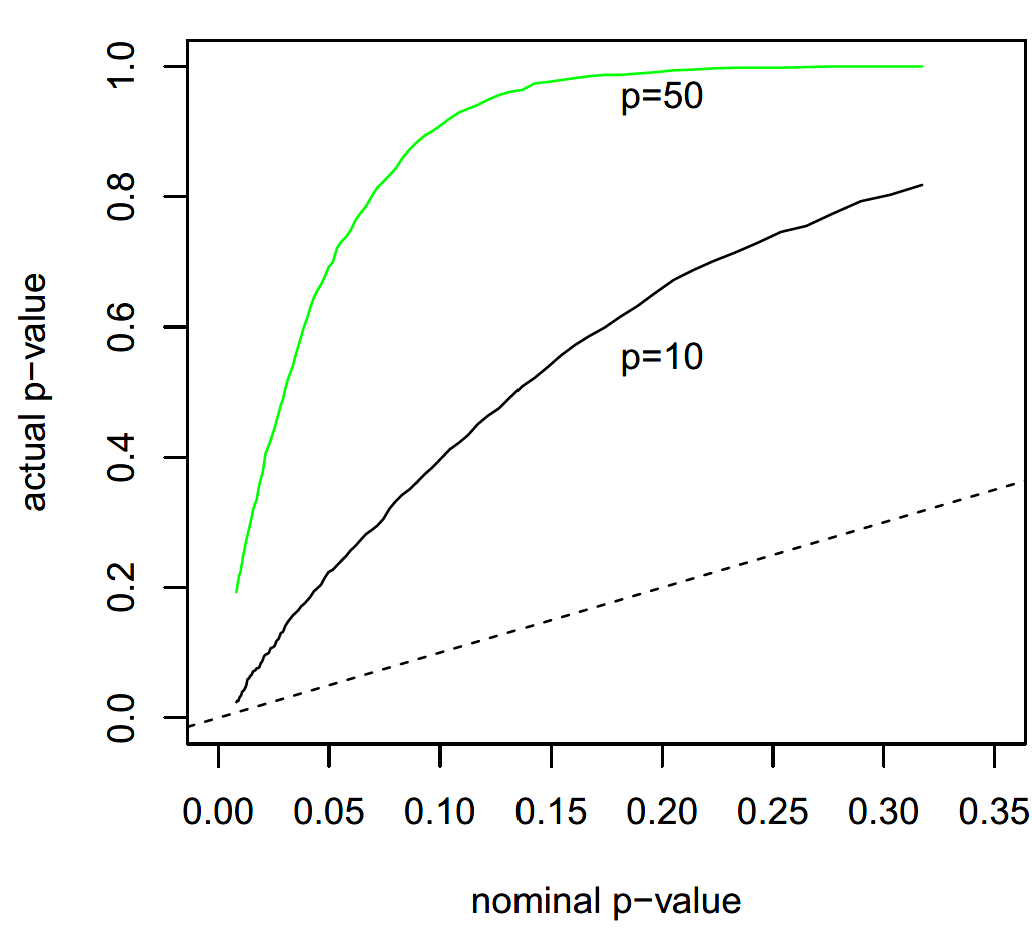
\includegraphics[width=0.6\linewidth]{stepwise_pvalue.png}
\end{figure}
\end{frame}

%------------------------------------------------
\begin{frame}
\frametitle{Forward Stepwise Regression}
\textbf{Example}: HIV data, $n=1073$ samples and $p=240$ mutation sites. Randomly select 100 samples and 30 sites. By forward stepwise regression, predictors enter in the order (5,9,25,8,16,21,...).
\begin{figure}
	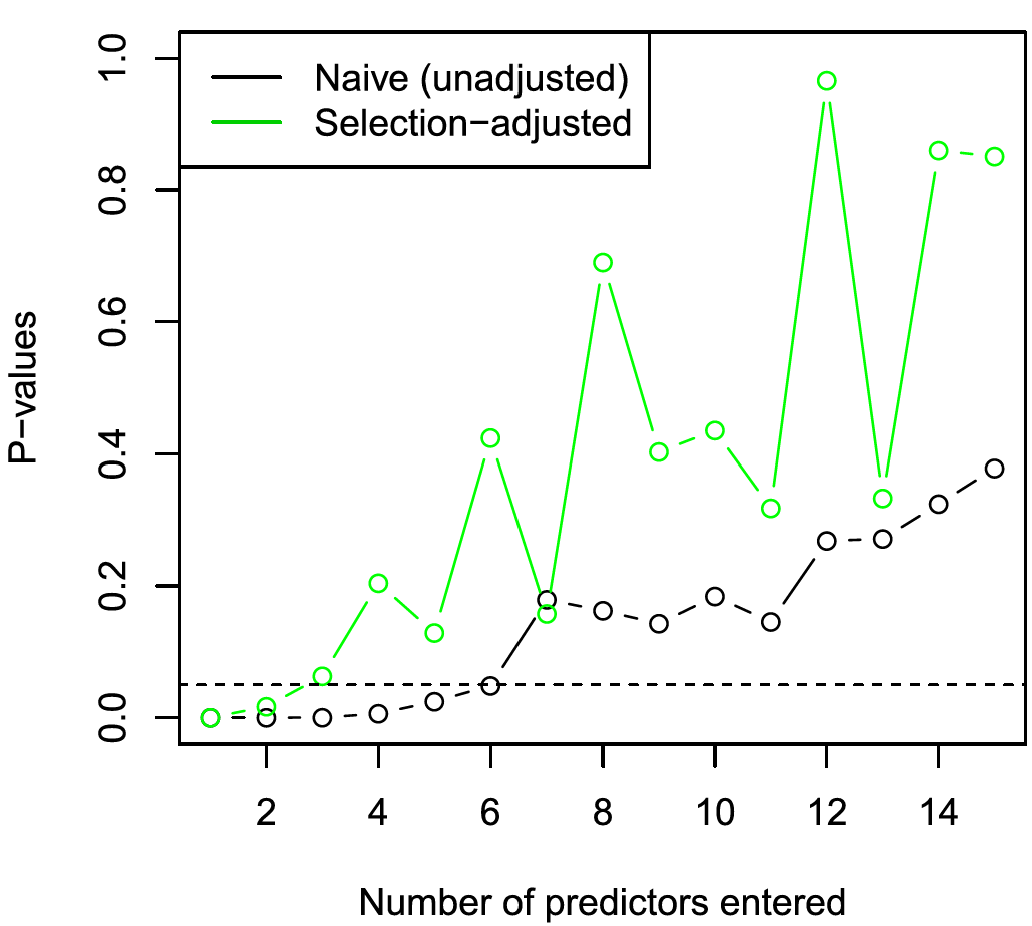
\includegraphics[width=0.6\linewidth]{stepwise_hiv.png}
\end{figure}
\end{frame}

%------------------------------------------------
\begin{frame}
\frametitle{Forward Stepwise Regression}
\begin{itemize}
	\item 
	Naive p-values $\Rightarrow$ 6 strong predictors
	\item
	After adjustment, only 2 or 3 are significant
	\item
	How to adjust? Do Monte Carlo directly? $\Rightarrow$ cumbersome
	\item
	Luckily, we can do things in closed form.
\end{itemize}
\end{frame}

%------------------------------------------------
\begin{frame}
\frametitle{Forward Stepwise Regression}
\begin{itemize}
	\item
	Assume have taken 2 steps, entering $x_5$ and $x_9$.
	\item
	standard: $\hat{\beta}\sim N(\beta, \tau^2)$. Assume we had only these 2 predictors available.
	\item
	This is not the case: select the strongest 2 from 30 predictors available.
	\item
	Write things in polyhedral form $Ay \leq b$. $A$ and $b$ depend on the data and selected variables.
	\item
	Each stage represents a competition among all $p$ variables. $A$ and $b$ reconstruct the competition and check whether new outcomes $y^*$ yields the same result.
	\item
	results of polyhedral selection: truncated normal $\hat{\beta}\sim TN^{c,d}(\beta, \tau^2)$
\end{itemize}
\end{frame}

%------------------------------------------------
\begin{frame}
\frametitle{Forward Stepwise Regression}
Truncated normal $\hat{\beta}\sim TN^{c,d}(\beta, \tau^2)$. $\hat{\beta}= 5.1$, $c = 4.3$ and $d = 6.3$.
\begin{figure}
	\makebox[\linewidth][c]{%
		\centering
		\subfigure[]{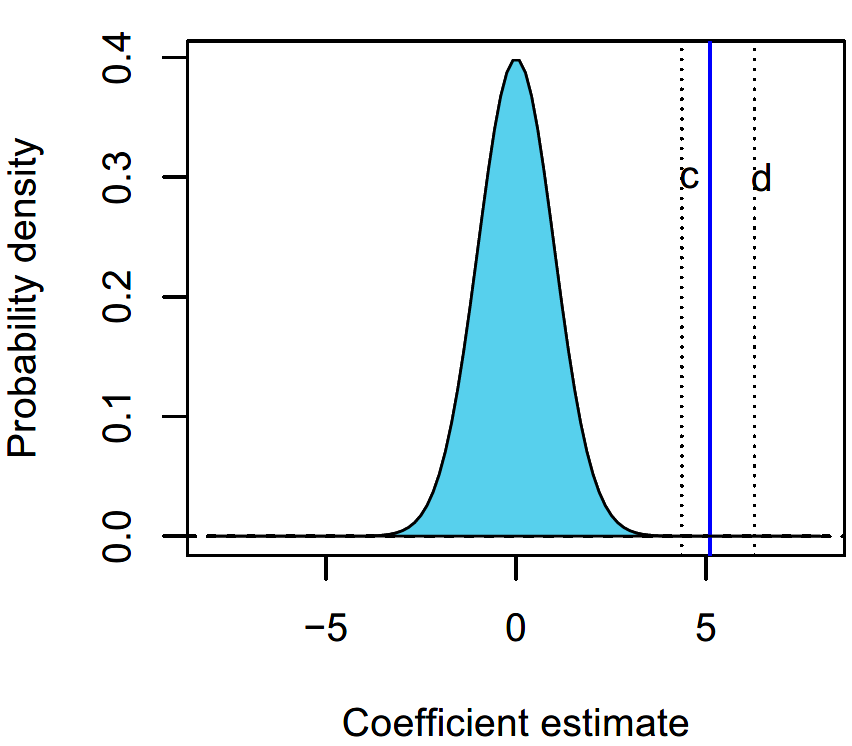
\includegraphics[width=0.4\textwidth]{stepwise_TN1.png}}%
		\subfigure[]{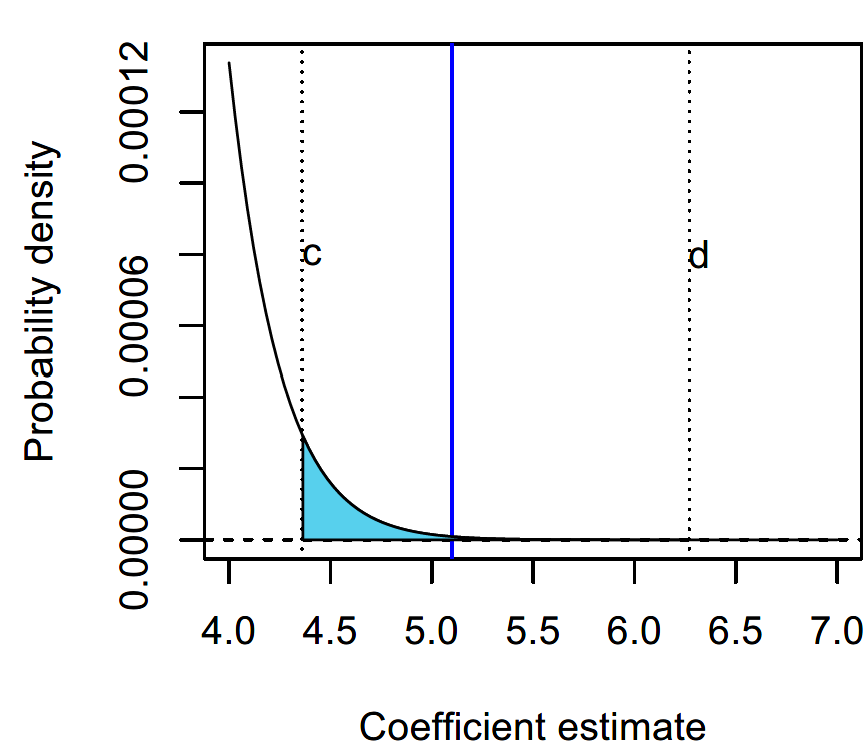
\includegraphics[width=0.4\textwidth]{stepwise_TN2.png}}%
	}
\end{figure}
Ignoring selection effects $\Rightarrow$ significant.\\
After adjustment $\Rightarrow$ moderate evidence
\end{frame}

%------------------------------------------------
\begin{frame}
\frametitle{FDR and Sequential Stopping Rule}
\textbf{Question}: when should we stop adding variables?\\
Control $FDR = E(V/R)$: $\hat{k} = max\{k: -1/k\sum_{i=1}^{k}{\log{1-pv_i}}\leq\alpha\}$, where $\{pv_i\}$ are successive p-values.
\begin{figure}
	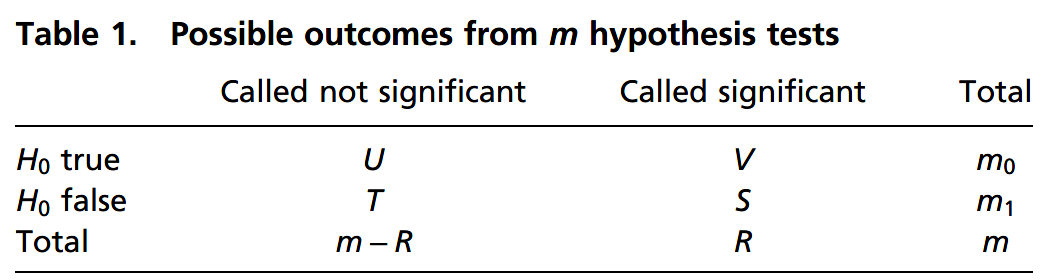
\includegraphics[width=0.6\linewidth]{stepwise_FDR.png}
\end{figure}
\end{frame}

%------------------------------------------------
\section{The LASSO}
%------------------------------------------------
\begin{frame}
\frametitle{The LASSO}
Modern approach for model selection: the LASSO
\begin{itemize}
	\item
	Still use the HIV data as an example.
	\item
	tune the parameter by cross-validation: 9 predictors
\end{itemize}
\begin{figure}
	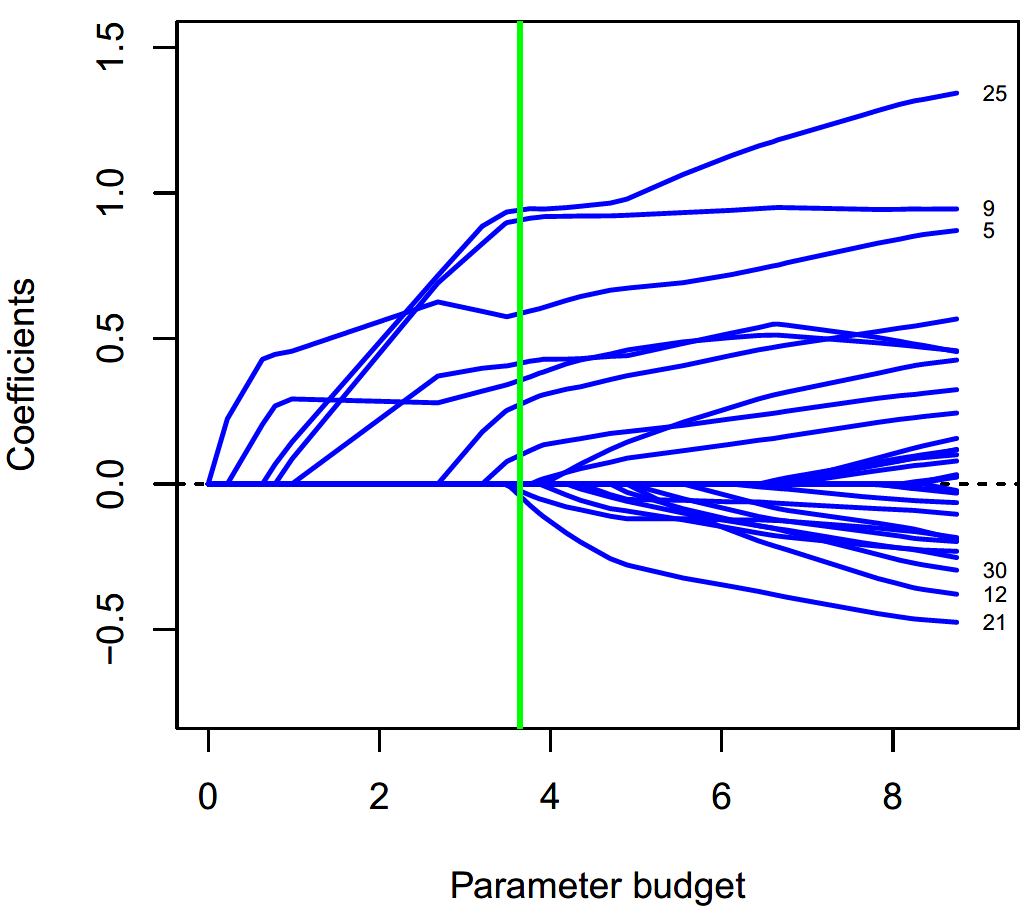
\includegraphics[width=0.6\linewidth]{lasso.png}
\end{figure}
\end{frame}

%------------------------------------------------
\begin{frame}
	\frametitle{The LASSO}
	Can still use the polyhetral region of the form $Ay \leq b$
	\begin{itemize}
		\item
		For fixed predictors and $\lambda$, the vector of response values $y^*$ that would yield the same active set can be written as $Ay^*\leq b$
		\item
		$A$ and $b$ depend on active set and $\lambda$, but not $y$.
		\item
		selection-adjusted intervals
	\end{itemize}
	\begin{figure}
		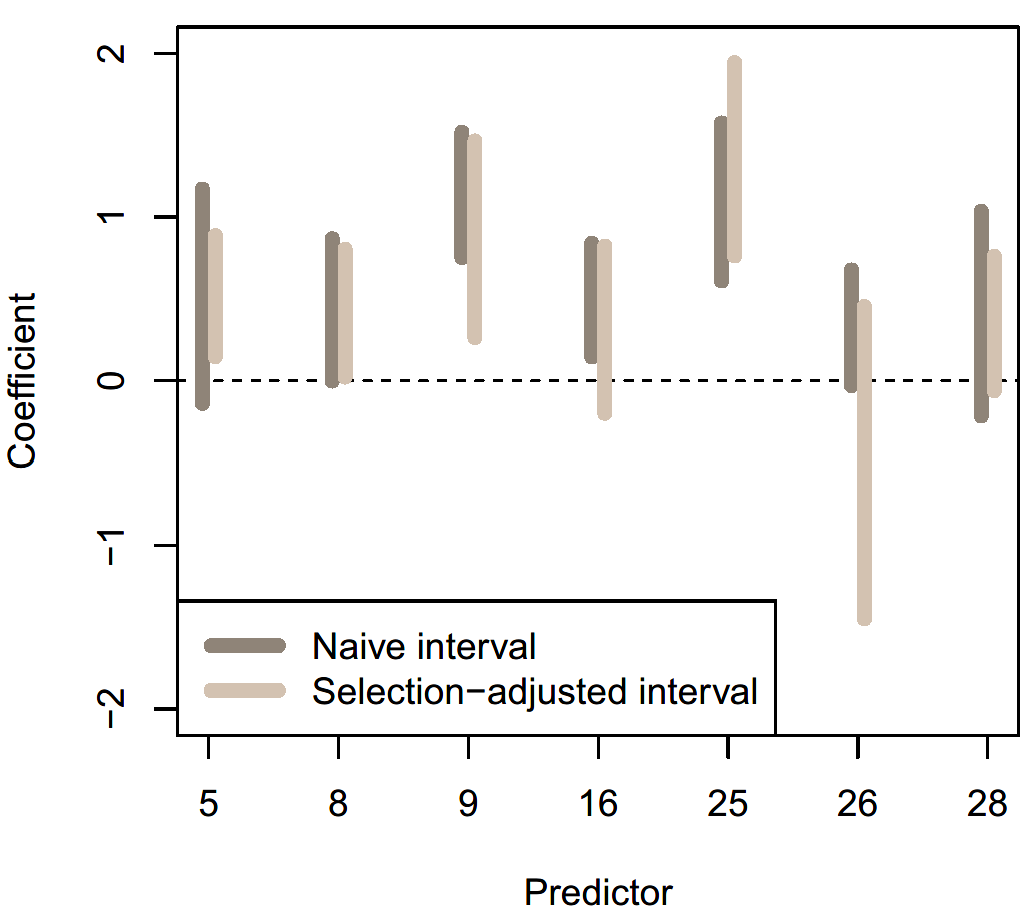
\includegraphics[width=0.5\linewidth]{lasso2.png}
	\end{figure}
\end{frame}

%------------------------------------------------
\section{PCA}
%------------------------------------------------
\begin{frame}
\frametitle{PCA}
How to select the number of components?
\begin{itemize}
	\item
	Traditional way: scree plot, based on the "elbow" point of eigenvalue
	\item
	But... It fails when there are too many noises.
	\item
	We can choose the leading eigenvectors as previous, i.e. calculate the adjusted p-values 
	\item
	calculate p-values is more informative: use more information in the correlation matrix, rather than just the eigenvalues. 
\end{itemize}
\end{frame}

%------------------------------------------------
\begin{frame}
\frametitle{PCA}
The adjusted p-values in the right: (0.030, 0.064, 0.222, 0.286, 0.197, 0.831, 0.510, 0.185, 0.126)
\begin{figure}
	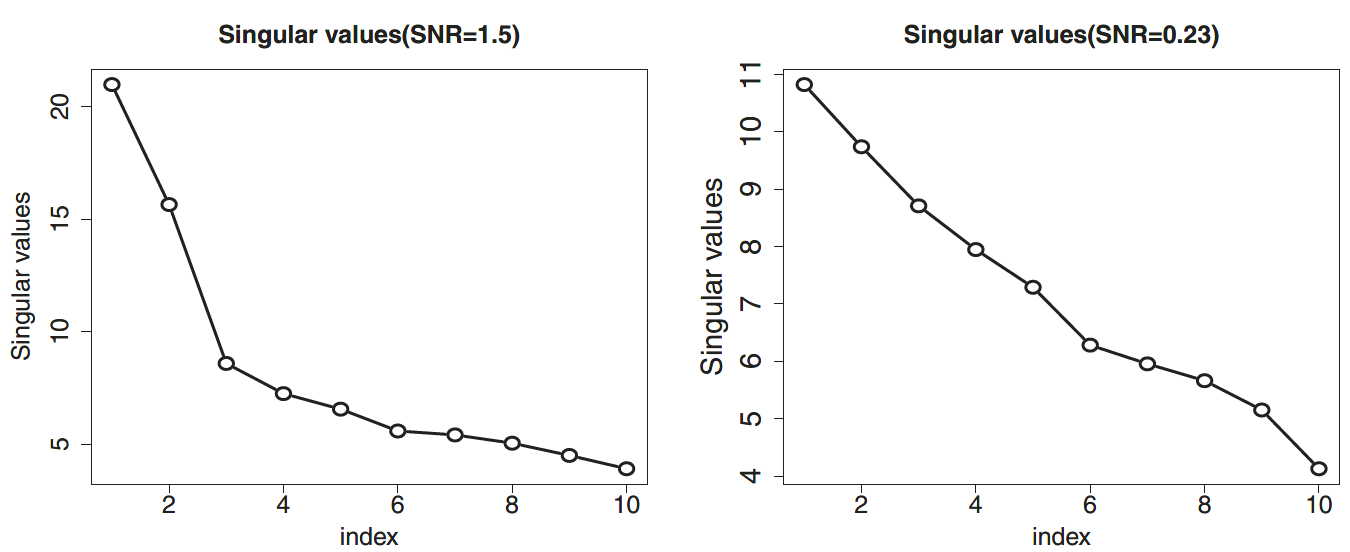
\includegraphics[width=0.8\linewidth]{pca.png}
\end{figure}
\end{frame}

\end{document}